\documentclass[letterpaper]{article}

% authors and affiliations
\title{Correlated movements can reshape spatio-temporal disease dynamics: modeling the contributions of space use to transmission risk using animal movement data}
\usepackage{authblk}
\author{Juan S. Vargas Soto, Lisa I. Muller, Dan Grove, Justin Kosiewska, and Mark Q. Wilber}
\affil{School of Natural Resources, University of Tennessee, Knoxville, TN}
\date{}


\usepackage[english]{babel}
\usepackage[utf8x]{inputenc}
\usepackage{amsmath}
\usepackage{graphicx}
\usepackage[left=1 in, right=1 in, top=1 in, bottom=1 in]{geometry}
\usepackage{hyperref}
\usepackage{bbold}
\usepackage{rotating}
\usepackage{bbm}
\usepackage{array}
\usepackage{xcolor}
\newcolumntype{C}[1]{>{\centering\arraybackslash}m{#1}}
% \usepackage{kbordermatrix}
\usepackage{footnote}
\makesavenoteenv{tabular}
\makesavenoteenv{table}
% \renewcommand{\theequation}{{S}\arabic{equation}}

\makeatletter
% \addto\captionsenglish{%
%   \renewcommand{\fnum@figure}{Figure S\thefigure}%
%   \renewcommand{\fnum@table}{Table S\thetable}%
% }
\makeatother

% Bibliography
\usepackage[round, colon]{natbib} % Bibliography - APA
\bibliographystyle{abbrvnat}
%\bibpunct{(}{)}{;}{a}{}{,}

% Line numbers
\usepackage{lineno}
%\def\linenumberfont{\normalfont\footnotesize\ttfamily}
%\setlength\linenumbersep{0.2 in}
\linenumbers

% Set space
\usepackage{setspace}
\doublespacing

% Command to e.g. write code that doesn't show up. Used as \ignore {some code}
\newcommand{\ignore}[1]{}

\begin{document}

\maketitle

\section*{Abstract}

\section*{Introduction}


%[Cite Das et al. 2023, Frontiers in Ecology and Evolution]

Individual movement is among the most critical factors that determine the dynamics of infectious disease in wildlife \citep{Dougherty2018,Manlove2022}. 
%For example, the combined dispersal of individuals in a population defines how parasites and infectious diseases spread across the landscape \citep{Fofana2017}. 
%At a more local scale, 
From an individual perspective, how an animal moves determines whether they encounter other individuals of the same species, other species, or parasites in the environment \citep{Martinez-Garcia2020,Das2023}. 
These encounters are a necessary component for the transmission of parasites and infectious diseases, and efforts have sought to identify where they could occur, how often, and how they could be influenced by environmental drivers \citep{Titcomb2021,Dougherty2022}. 
Being able to formally link environmental factors, animal movement, contact, and parasite transmission risk, could improve our ability to predict and prevent outbreaks and would represent a significant advancement for management of wildlife diseases.  
Nevertheless, understanding and extrapolating the relationships between these processes at an individual scale requires extremely detailed information about movement, combined with analytical frameworks that can translate this information into an epidemiological context.

Recent approaches developed at the interface of movement and disease ecology are able to leverage animal tracking data with high spatial and temporal resolution to gain insight into contact among individuals and disease transmission \citep{Wilber2022,Yang2023}. For example, movement-driven modeling of spatio-temporal infection risk (MoveSTIR) builds dynamic spatio-temporal contact networks from which we can estimate the risk of infection for different individuals across space and time \citep{Wilber2022}. MoveSTIR provides a theoretical foundation to translate contacts observed or inferred from spatial data into the epidemiological currency of force of infection, which represents the risk of transmission experienced by a host per unit time. These studies have highlighted the importance of individual heterogeneity and temporal scale for disease dynamics, particularly how indirect contact---two individuals at the same place at different times---can significantly reshape contact and transmission networks \citep{Richardson2015,Wilber2022,Yang2023}. These approaches are nonetheless based on occurrence, rather than range, distributions \citep[in the terminology of ][]{Alston2022} -- meaning it only considers where animals were observed and not where they \emph{potentially} could have moved. This makes it difficult to systematically link observed encounters with underlying spatial covariates, and to predict how social or environmental changes affect contact and transmission. 

An alternative approach would be to use utilization distributions (UDs) to infer spatial and temporal contact and transmission probabilistically. An individual's UD is defined as the probability---either transient or in the long-run \citep{Tao2016}---that it uses a particular area on a landscape, and is perhaps the best representation of the long-term relationship between environment and use of space over different time scales \citet{Webber2023}. The high spatial and temporal resolution of modern tracking data serves to build UDs based on biologically realistic movement models \citep{Fleming2014,Gurarie2011,Potts2023}, and to link them with underlying resources [citations].
Individually defined UDs can be combined to study pairwise interactions, for example to quantify the degree of overlap between home ranges \citep{Winner2018}, or to estimate the expected location and rate of encounter between individuals  \citep{Noonan2021}, which could be used to infer contact and transmission \citep{Godfrey2010, Godfrey2013,Noonan2021}. 
Moreover, because UDs can be directly linked to environmental drivers of movement \citep{Signer2017}, they have the potential to predict contact and transmission in novel environments and can also be used for prospective analyses to understand how the effects of environmental and social perturbations cascade across scales, from individual movement to population and landscape-level disease transmission. 

Current contact metrics based on UDs focus only on direct interaction, ignoring temporal dynamics that are especially relevant for epidemiological processes. The Conditional Distribution of Encounters (CDE) \citep{Noonan2021}, for example, estimates the probability that two individuals will come into contact with each other at a given location, assuming that individuals move independently from each other.
While a useful simplification, social interactions like territoriality or gregariousness can invalidate this assumption \citep{Manlove2018,Sah2018}. In these cases, temporal correlations in space use could increase or decrease the expected probability of encounter compared to an assumption of independent movement \citep{Kjaer2008,Schauber2015a}. 
Moreover, direct interactions do not necessarily equate to \emph{epidemiological contacts}, which consist of contact formation, contact duration, pathogen acquisition, pathogen shedding, and pathogen decay. As some parasites can persist in the environment for months or years (e.g. anthrax, CWD), ignoring these processes could severely underestimate the risk of transmission \citep{Wilber2022,Yang2023,Richardson2015}.

In general, we lack a way to quantify the role of social interactions on spatio-temporal force of infection, which limits our ability to assess when ignoring correlated movements actually matters when assessing infection risk. One of our goals in this study is to ask: how much can correlated, social movements affect spatio-temporal infection risk for directly and indirectly transmitted pathogens? A large portion of epidemiological theory is built upon the assumption of independent host movements in the presence of absence of spatial heterogeneity, but there is very little theory that quantifies how correlated movements affect contact and transmission risk.  In contrast, there is a large body of empirical work that empirically quantifies how correlated and social movements can reshape contact and transmission landscapes \citep{Kjaer2008,Grear2010,Schauber2015a,Webber2023} [other citations from non-deer systems needed].  Bridging this gap from what we observe empirically to what we expect theoretically is a key missing link. While MoveSTIR implicitly accounts for such correlations, it only applies for observed data. In contrast, the CDE provides a basis for estimating encounter probabilities across the landscape, but ignores correlations and temporal dynamics of indirect contact.
Ultimately, an approach is needed that combines the range-distribution inference of UDs and CDEs \citep{Alston2022,Noonan2021} with the epidemiological focus of MoveSTIR to link UDs to epidemiological dynamics. 

Here, we develop a model we refer to as Probabilistic MoveSTIR (PMoveSTIR) to estimate epidemiological contact and expected force of infection across space and time from UDs. Our approach provides probabilistic, spatio-temporal contact networks that can be used to predict out-of-sample transmission risk under independent movements. We first derive the most general PMoveSTIR model using transient UDs and then provide different modifications to consider heterogeneities in space and time. We show how PMoveSTIR encompasses other common assumptions such as mass action transmission and home range overlap transmission as special cases. Deriving analytical results and applying PMoveSTIR to simulated movement data, we demonstrate the sometimes sizable importance of non-independent movements on pairwise transmission risk, indicating that ignoring the social drivers of contact could severely bias epidemiological inference. However, our simulations show that this result primarily holds for directly transmitted parasites. For parasites that persist for long periods of time in the environment, non-independent host movements are largely inconsequential compared to spatial overlap for transmission risk. We demonstrate this result empirically using a dataset of white-tail deer movements and show that empirically observed correlated movements can increase potential force of infection by orders of magnitude for a hypothetical directly transmitted parasite but are relatively unimportant for a hypothetical parasite with long persistence times.  Overall, PMoveSTIR is a critical next step for developing predictive models that link movement data to spatio-temporal infection dynamics on real landscapes.

\section*{Methods}

\subsection*{Model development - Linking utilization distributions to transmission through PMoveSTIR}

PMoveSTIR builds on the recently developed MoveSTIR model \citep{Wilber2022} and formally links host utilization distributions, direct and indirect contacts, correlated animal movements, and spatial estimates of force of infection (FOI). This an essential quantity in disease ecology that underlies our ability to predict the spread of disease across populations and landscapes. Essentially, we want to know, for two individuals $i$ and $j$ moving and interacting across a landscape, what is the FOI host $i$ experiences from host $j$, across space and time?  

As in MoveSTIR, we assume that transmission happens by an infected host depositing pathogen into the environment and another host picking that pathogen up. 
Deposition and acquisition can represent a range of processes, from one individual coughing and another inhaling in a matter of seconds, to one host depositing parasite eggs or larvae in the environment and another individual consuming these days or weeks later. 
This fairly general assumption encompasses standard density-dependent transmission as a special case \citep{Cortez2021}. 
Moreover, considering transmission through deposition and acquisition components clearly links direct transmission and indirect transmission along a continuum \citep{Wilber2022}.

In PMoveSTIR, we assume a ``contact'' can occur if both individuals visit a given location $x$, which could be a habitat patch or a grid cell. 
For the results we discuss in the main text, we assume that locations $x$ on the landscape do not overlap such that summing the areas of locations $x$ equals some total area over which individuals can move (in Appendix 1 we provide a derivation when $x$ is a point, not an area, on the landscape). 
Furthermore, we assume that the likelihood of contact is uniform within the location $x$, consistent with a so-called top-hat encounter function \citep{Gurarie2013,Wilber2022}.

Given these assumptions, we can define the pairwise force of infection felt by host $i$ from host $j$ in location $x$ at time $t$ as \citep{Wilber2022}
\begin{equation}
    h_{i \leftarrow j}(t, x) = \int_{-\infty}^{t} \beta' \lambda \delta_{x_j(u)}(x) \delta_{I_j(u)}(I) S(t - u) du
    \label{eq:original_foi}
\end{equation}
where $\lambda$ is the pathogen deposition rate of host $j$, $\delta_{x_j(u)}(x)$ is an indicator variable that is one if host $j$ is in location $x$ at time $u$ and zero otherwise, $\delta_{I_j(u)}(I)$ is an indicator function that is one if host $j$ is in an infected state at time $u$ and zero otherwise, and $S(t-u)$ is the probability that any pathogen deposited at time $u < t$ is still alive at time $t$ \citep[see][for a full derivation]{Wilber2022}. 
The term $\beta'$ is the rate at which host $i$ picks up pathogen within the location $x$ and can be re-written as $\tilde{\beta} / A_x$, where $\tilde{\beta}$ can be considered a ``search efficiency'' term, with units area/time (e.g., $m^2 / day$), and $A_x$ gives the area of location $x$ (e.g., 100 $m^2$). 
Therefore, the total acquisition rate scales with the area in which contact can occur; in larger areas, the acquiring host would have to search for longer to find a ``packet'' of pathogen, reducing the host's total acquisition rate and the corresponding FOI. Moving forward, we assume that host $j$ (the depositing host) is always infected.  This is equivalent to building a contact network and also represents the structural form of FOI needed to compute pathogen invasion thresholds \citep{Wilber2022}.

Considering probabilistic movements (i.e., we only know where an individual is with some probability at a given time), we can then re-write equation \ref{eq:original_foi} as
\begin{equation}
    h_{i \leftarrow j}(t, x) = \int_{-\infty}^{t} \beta' \lambda \delta'_{x_i(t)}(x) \delta'_{x_j(u)}(x) S(t - u) du
    \label{eq:prob_foi}
\end{equation}
where $\delta'_{x_i(t)}(x)$ and $\delta'_{x_j(u)}(x)$ are random variables that specify whether or not (i.e., 0 or 1) host $i$ or host $j$ is in location $x$ at time $t$.  This means that $h_{i \leftarrow j}(t, x)$ is also a random variable, and we can express its expected value as 
\begin{equation}
    E[h_{i \leftarrow j}(t, x)] := h^*_{i \leftarrow j}(t, x) = \int_{-\infty}^{t} \beta' \lambda E[\delta'_{x_i(t)}(x) \delta'_{x_j(u)}(x)] S(t - u) du.
    \label{eq:expected_foi}
\end{equation}
Interpreting this expectation, we are asking: if we simulated some movement process thousands of times, what is the probability that host $i$ is in location $x$ at time $t$ and host $j$ was in location $x$ at a previous time $u$? 

\subsubsection*{Linking equation \ref{eq:expected_foi} to utilization distributions}

Note that for two random variables $Y$ and $Z$, we have $E[YZ] = E[Y]E[Z] + Cov(Y, Z)$.  We can therefore write equation \ref{eq:expected_foi} as
\begin{equation}
    \begin{aligned}
        h^*_{i \leftarrow j}(t, x) &= \int_{-\infty}^{t} \frac{\tilde{\beta}}{A_x} \lambda E[\delta'_{x_i(t)}(x) \delta'_{x_j(u)}(x)] S(t - u) du \\
        &= \frac{\tilde{\beta}}{A_x} \lambda \int_{-\infty}^{t} [E[\delta'_{x_i(t)}(x)] E[\delta'_{x_j(u)}(x)] + Cov(\delta'_{x_i(t)}(x), \delta'_{x_j(u)}(x))] S(t - u) du \\
        &= \frac{\tilde{\beta}}{A_x} \lambda \int_{-\infty}^{t} [p_i(x, t) p_j(x, u) + Cov(\delta'_{x_i(t)}(x), \delta'_{x_j(u)}(x))] S(t - u) du \\
    \end{aligned}
    \label{eq:foi_cov}
\end{equation}
where we use the fact that the expectation of an indicator variable is a probability \citep{Grimmett2001}. The terms $p_i(x, t)$ and $p_j(x,u)$ give the probabilities that host $i$ and $j$ are in location $x$ at times $t$ and $u$, respectively, and can also be written as $p_i(x, t) = \int_{A_x} f_i(s, t) ds$ where $f_i(s, t)$ is the probability density of host $i$ using the point $s$ at time $t$ and the integral is over the area $A_x$ (defined equivalently for host $j$). Thus, we have obtained an equation that links the transient utilization distributions $f_i(s, t)$ and $f_j(s, u)$ with the spatio-temporal FOI.

\subsubsection*{Applying the PMoveSTIR framework under different degrees of spatial and temporal heterogeneity}

Equation \ref{eq:foi_cov} is the most general formulation of PMoveSTIR, where utilization distributions and between-individual spatial covariance are time-varying and heterogeneous in space. For example, this could account for daily changes in habitat use and social interactions. The approach can be modified to consider different degrees of spatial and temporal heterogeneity. This allows us to link FOI to different metrics such as temporally varying utilization distributions, stationary utilization distributions, and home range overlap. 

Fig. \ref{fig:square} shows the different scenarios that PMoveSTIR can consider. In the upper-left corner, we consider space use is uniform, but movement is non-stationary. In this case, it is not important where an individual is, just when. Considering this framing from an empirical point of view, proximity loggers deployed on individual hosts --- a commonly used tool to measure among-animal contacts \citep{Drewe2012} --- only tell us when contacts between individuals occur, but not where.  Thus, we cannot make inference about spatial factors driving contacts, but can make inference on temporal processes.  We consider this case in a future study.

In the lower left-hand corner of Fig. \ref{fig:square}, we have the case where space use is uniform and time is stationary. For simplicity, we also assume that pathogen decay is exponentially distributed with a rate of decay $\nu$ such that $S(s) = \exp(-\nu s)$. Given these assumptions, we can write the FOI equation as
\begin{equation}
    \begin{aligned}
        h^*_{i \leftarrow j}(A_x) = \beta' \lambda \left[\frac{A_x}{A_{tot}}\frac{A_x}{A_{tot}} \frac{1}{\nu} +  \int_{0}^{\infty} Cov(\delta_{i \in A_x}, \delta_{j \in A_x} | s) e^{-\nu s} ds\right]
    \end{aligned}
    \label{eq:uniform_stationary1}
\end{equation}
where the covariance in contact is constant across all areas $A_x$ on the landscape (such that $\delta_{i \in A_x}$ indicates the use of some arbitrary area $A_x$).  
If hosts are moving independently (i.e., covariance is 0) we obtain $\frac{\tilde{\beta}}{A_x} \frac{A_x}{A_{tot}} \frac{A_x}{A_{tot}}  \frac{\lambda}{\nu}$. Given a gridded landscape with non-overlapping grids and $x$ is a single grid cell, summing over all $n$ areas $A_x$ that comprise the landscape yields $\bar{h}_{i \leftarrow j} =\frac{\tilde{\beta}}{A_\text{tot}} \frac{\lambda}{\nu}$, which is the standard mass action assumption of transmission \citep{McCallum2001}. 

Finally, the lower-right corner represents the special case of statistical stationarity in movement (i.e., the mean location is constant through time, though the animal is still moving).
Again assuming that pathogen survival in the environment follows $S(s) = e^{-\nu (s)}$, where $\nu$ is a constant pathogen decay rate,  we can simplify equation \ref{eq:foi_cov} to (derivation in Appendix 2)
\begin{equation}
    \begin{aligned}
   h^*_{i \leftarrow j}(x) = \frac{\tilde{\beta}}{A_x} \lambda \left[p_i(x)p_j(x) \frac{1}{\nu} + \int_{0}^{\infty} Cov(\delta_{i \in x}, \delta_{j \in x} | s) e^{-\nu s} ds\right]
    \end{aligned}
    \label{eq:foi_stationary}
\end{equation}
The key insight here is that, given a stationarity assumption, the expected force of infection in location $x$ depends on i) the marginal probabilities that host $i$ and host $j$ use location $x$ (i.e. their UDs),  and ii) the covariance in how host $i$ and host $j$ use location $x$, integrated over different time lags $\tau$. 
To improve intuition, we can redefine $Cov(\delta_{i \in x}, \delta_{j \in x} | s) = \sigma_i(x) \sigma_j(x) Cor(\delta_{i \in x}, \delta_{j \in x} | s)$, where $\sigma_i(x) = \sqrt{p_i(x)(1 - p_i(x))}$  and $\sigma_j(x) = \sqrt{p_j(x)(1 - p_j(x))}$ are the standard deviation in probability of host $i$ and $j$ using location $x$, respectively.  We can then write
\begin{equation}
    \begin{aligned}
    h^*_{i \leftarrow j}(x) = \beta' \lambda [ \underbrace{p_i(x)p_j(x) \frac{1}{\nu}}_{\substack{\text{FOI contribution from} \\ \text{shared space use}}} + \sigma_i(x) \sigma_j(x) \underbrace{\int_{0}^{\infty} Cor(\delta_{i \in x}, \delta_{j \in x} | s) e^{-\nu s} ds]}_{\substack{\text{FOI contribution from} \\ \text{correlated movement}}}.
    \end{aligned}
    \label{eq:stationary_cor}
\end{equation}
Equation \ref{eq:stationary_cor} highlights that the key quantity we need to understand is the correlation in host $i$'s and host $j$'s use of location $x$ at different time lags $s$, i.e. the temporal cross-correlation in space use.
This correlation is most easily understood for short time lags ($s\approx0$), for which a positive value indicates that individuals are at the same location at the same time or one shortly after the other. In contrast, negative correlations at short lags indicate the individuals rarely encounter each other directly.
In what follows, we focus on this case and explore how and under what circumstances correlated movement can influence the FOI. We analyze different scenarios of movement analytically, using simulations, as well as empirical data.  In Appendix X, we examine a two additional formulations of PMoveSTIR that highlight the flexibility of this approach for linking range distributions (including home ranges and UDs) and spatial-temporal infection risk.

\subsection*{Analytical and simulation insight into correlated movement and FOI}

Leveraging PMoveSTIR, we used analytical analysis, simulation, and empirical data to ask: how much can correlated, social movements affect spatio-temporal infection risk for directly and indirectly transmitted parasites? 
First, we used PMoveSTIR to derive a general formula that explicitly quantifies how much correlation can augment or reduce force of infection due to direct contact compared to random movement. We also derived analytical results for a specific movement pattern to demonstrate how correlated movements alter transmission risk due to indirect transmission.
Second, we used simulations to explore how temporally correlated movements affect  transmission, and how the pairwise FOI estimate depends on epidemiological parameters such as contact distance and parasite survival. We focus on the lower-right corner of the PMoveSTIR box (eq. \ref{eq:stationary_cor}), where we assume statistical stationarity in movement. The process for calculating the FOI across the landscape is summarized in Fig. \ref{fig:steps}.

In every simulation, we have two individuals moving around established home ranges, according to an Ornstein-Uhlenbeck process. To create different levels of correlation, we modify the initial simulated tracks using a convolution approach with a social interaction kernel \citep{Scharf2018}. This method accounts for constant or temporally varying attraction between pairs of individuals. For our purposes we assume attraction strength is constant in time, but varies across pairs from 0 (completely independent movement) to 1 (joint movement). Strong interactions lead to similar and highly overlapping trajectories, which could represent animals in a herd, courting/mating pairs, or parents with their offspring.
For every scenario, we fit continuous-time movement models to the simulated tracks, and estimate individual UDs using autocorrelated kernel density estimation \citep{Calabrese2016}. We estimate the UDs on a grid of square cells, where the cell side $d$ is the threshold contact distance for epidemiological contact. 

We use the UDs to calculate the product of the probabilities of use ($p_i(x)p_j(x)$) and the product of their standard deviations ($\sqrt{p_i(x)(1-p_i(x))}\sqrt{p_j(x)(1-p_j(x))}$) for each grid cell.
The UD product represents the overlap between home ranges, and is related to the probability of encounter between individuals \citep{Noonan2021}. Assuming we are integrating over infinite lags, we can scale the UD product by $1/\nu$ to obtain the first term in brackets on the right hand side of equation eq. \ref{eq:stationary_cor}. In practice we will actually have a limited time given by the data, which sets an upper limit on the lags that can be considered. If this time is short relative to the parasite decay function there could be substantial error in the estimation. A more formal approach is then to use the integral over a specific period  $\int_0^{\tau} e^{-\nu s}ds=(1-e^{-\nu\tau})/\nu$.
 Both products are symmetrical for every pair of individuals. 

The lagged correlation term is calculated based on the position history for each individual at locations that both visited (locations that only one or neither individual visited have a correlation of zero). This is a binary vector that specifies whether the individual was present (1) or absent (0) at location $x$ at time $t$. 
The order of visits matters, so these correlation values can be asymmetric between individuals. 
We then scale the correlation values by $e^{-\nu\tau}$ due to the decay of the parasite, where $\tau$ is the lag corresponding to each cross-correlation, between 0 and $t-dt$, where $dt$ is the (constant) time lag between measurements. 

Substituting the terms in eq.\ref{eq:stationary_cor} and scaling by the epidemiological parameters $\tilde\beta\lambda/ A_x$ we obtain the per-cell FOI. Through these simulations we explore how the expected FOI is influenced by correlation in space use, home range overlap, parasite decay rate, and contact distance. We also explore how the contribution from the correlation to the total and local FOI varies. 

% Because Negative correlation terms could occasionally make a cell's estimated FOI negative, especially for small cells where the probabilities of use are low; the FOI is nevertheless strictly positive by definition, so in these cases we set the cell FOI to zero.

\subsection*{Empirical application - White-tailed deer}

To test the role of space-use and correlated movements on potential transmission risk in a real system, we applied the PMoveSTIR model to GPS-tracking data for five white-tailed deer (\emph{Odocoileus virginianus}) from Ames Plantation, Tennessee, USA (two bucks and three does).%JUAN here: I changed the individuals to get a longer period of overlap. I removed 64, please check that the sexes are still correct.
Deer were capture and equipped with GPS collars that recorded fixes every 30 minutes (Lotek LifeTrack IR 420; IACUC \# 2850-1021 from the University of Tennessee).  All individuals used in this study were captured at the end of March 2023 and we only included movement data from May to June in this study (removing April data to eliminate any capture effects on movement).  We fit continuous-time movement models to each track and estimated the utilization distributions (UD) using AKDEs \citep{Calabrese2016}. We defined a contact as occurring when hosts occupied the same 10m by 10m square cell.  Using the fitted continuous-time movement model for each individual, we interpolated the positions to regular 10 minute intervals to account for missed fixes, \citep{Yang2023}. 

We modeled two hypothetical pathogens. The first pathogen had a relatively short persistence time in the environment, surviving for an average of 1 hour  ($\nu=1 h^{-1}$). In this case, transmission is largely direct and this might represent a pathogen like SARS-COV-2,  which can infect and transmit between white-tailed deer [citations]. The second hypothetical pathogen had a long persistence time, remaining viable for over a year on average ($\nu=0.9 yr^{-1}$). In this case, transmission is largely indirect and might reflect a pathogen like chronic wasting disease \citep[CWD][]{}.  Chronic wasting disease can transmit directly and indirect between deer and can persist for years in the environment [citations]. The $\beta$ and $\lambda$ parameters are scalars in PMoveSTIR and do not affect any relative comparisons, so we set them both to unity. 
We use these data to explore how differences in overlap across home ranges and  correlated movement influence the expected FOI with real animal trajectories.

\section*{Results}

\subsection*{The importance of correlated movements on FOI -- analytical results}

To gain analytical intuition into the role that correlated movement can have on FOI, consider equation \ref{eq:uniform_stationary1} where movement is statistically stationary and hosts use space uniformly.  As we showed above, when correlation in movement is zero, equation \ref{eq:uniform_stationary1} reduces to mass action transmission. 
For illustrative purposes, consider a case where two individual hosts are moving together across some area $A_{tot}$. We assume that hosts spend $\eta$ time units within a habitat patch/grid cell of area $A_x$ before moving to the next patch/grid cell. Second, we assume that the pathogen survival function $S(s)$ is a step function with a survival probability of one when lag $s \leq \pi \eta$ and zero when $s > \pi \eta$.  
The term $\pi \eta$ gives the time the pathogen survives in the environment as a function of host residence time, where $\pi$ ranges from near zero for directly transmitted pathogens to some arbitrarily large number for pathogens with long environmental persistence times.  
In this scenario, transmission can only occur while both animals are in the same patch. With these assumptions, we can rewrite equation \ref {eq:uniform_stationary1} as 
\begin{equation}
    \begin{aligned}
        h^*_{i \leftarrow j}(A_x) = \beta' \lambda \left[\frac{A_x}{A_{tot}}\frac{A_x}{A_{tot}} \pi \eta + \frac{A_x}{A_{tot}}(1 - \frac{A_x}{A_{tot}}) \int_{0}^{\pi \eta} Cor(\delta_{i \in A_x}, \delta_{j \in A_x} | s) ds\right],
    \end{aligned}
    \label{eq:uniform_stationary2}
\end{equation}
recognizing that $\sigma_i(x) \sigma_j(x) = \sqrt{\frac{A_x}{A_{tot}}(1 - \frac{A_x}{A_{tot}})}\sqrt{\frac{A_x}{A_{tot}}(1 - \frac{A_x}{A_{tot}})} = \frac{A_x}{A_{tot}}(1 - \frac{A_x}{A_{tot}})$ when both hosts are using space uniformly.

\subsubsection*{Direct transmission}

For hosts that are moving together, $Cor(\delta_{i \in A_x}, \delta_{j \in A_x} | s)$ will be exactly unity when lag $s = 0$ and near unity when lag $s$ is near zero. When pathogens are strictly directly transmitted, $\pi$ is also small and if $\pi \eta << \eta$ then we can reasonably approximate $Cor(\delta_{i \in A_x}, \delta_{j \in A_x} | s) = 1$ for s from 0 to $\pi \eta$.  We can then write equation \ref{eq:uniform_stationary2} as 

\begin{equation}
    \begin{aligned}
        h^*_{i \leftarrow j}(A_x) = \beta' \lambda \pi \eta \left[\underbrace{\frac{A_x}{A_{tot}}\frac{A_x}{A_{tot}}}_{\substack{\text{Contribution due} \\  \text{to habitat overlap}}} + \underbrace{\frac{A_x}{A_{tot}}(1 - \frac{A_x}{A_{tot}})}_{\substack{\text{Contribution due} \\ \text{to correlated movement}}} \right].
    \end{aligned}
    \label{eq:uniform_direct}
\end{equation}
The relative contribution of correlation in movement with respect to the contribution due to habitat overlap is simply $(1 - (A_x / A_{tot})) / (A_x / A_{tot})=A_{tot}/A_x-1$. 
Thus, PMoveSTIR allows us to put intuitive bounds on the importance of correlated movements for direct transmission risk. 
As the area $A_x$ in which an epidemiological contact can occur gets smaller relative to the total area in which the hosts are moving $A_{tot}$, the correlated movement can have an orders of magnitude larger contribution to direct transmission FOI than habitat overlap at the scale of the area $A_x$. If there are large  correlations across multiple areas this will add up into a significantly greater FOI across the entire landscape.
This makes intuitive sense. If the area of potential contact is small and hosts are moving randomly, there is a very low chance that hosts will be there together at the same time.  Having highly correlated movements significantly increases the chance that hosts are in this relatively small area at the same time.  
In contrast, when the area of contact $A_x$ approaches $A_{tot}$ (or more generally when the probability of using a particular area is very high), the importance of correlated movement relative to habitat overlap becomes minimal. For example, if two hosts are always using a particular contact area together because of high resource availability, then it does not matter for FOI if social factors are leading to additional correlated movement. This result extends beyond epidemiological contexts and shows when correlated movements can significantly alter contact risk based on metrics such as home range overlap or CDE.

\subsubsection*{Indirect transmission}

The effects of correlated movement on FOI relative to habitat overlap become analytically more difficult to generalize when we consider pathogens with indirect transmission.  This is because the correlation function $Cor(\delta_{i \in A_x}, \delta_{j \in A_x} | s)$ can be highly non-trivial even in the simple case when two hosts are moving together. For example, even individuals that never encounter each other directly can have positive correlations at relatively short lags, and these can be greater than the correlations for individuals that do come into direct contact but only overlap partially at the same locations (Fig. \ref{fig:xcorrs}b,c).
While determining the analytical form of $Cor(\delta_{i \in A_x}, \delta_{j \in A_x} | s)$ for common movement models is beyond the scope of this study, we can use a relatively simple movement scenario to get an analytical sense of how indirect transmission and correlated movements can interact to affect transmission risk.  We provide the analytical example in Appendix S3. The example illustrates three important points: 1) the contributions of correlated movement to indirect transmission risk will depend strongly on the movement dynamics as reflected in $Cor(\delta_{i \in A_x}, \delta_{j \in A_x} | s)$; 2) this contribution could potentially increase, decrease, or have no effect on local FOI depending on the lag considered; 3) the relative importance of correlations at different lags is determined by the parasite survival function.
Below, we explore these factors using simulations.

\subsection*{Simulation study}

%The overall FOI varied more than four orders of magnitude among simulations, in response to both movement and epidemiological parameters. 
\subsubsection*{Effect of correlated movement on pairwise FOI}

Generally, greater interaction strengths led to higher overlap among home ranges. Simulations with interaction strengths greater than 0.9 all resulted in overlap values greater than 0.99, meaning the utilization distributions were always virtually identical. Pairs moving independently had lower overlap values on average but also higher variance, so in many cases had similarly high overlap ($>$0.9). This allows us to compare the FOI while teasing apart the effects of spatial overlap and temporal correlation in space use. 

The FOI was higher for pairs with higher interaction strengths, i.e. pairs that were more attracted to each other. This increase was due in part to higher spatial overlap, as can be seen from the higher FOI values calculated using only the stationary utilization distribution component (Fig. \ref{fig:simresults}a). However, we saw a greater increase in FOI when we accounted for temporal correlation, and the difference between the two increased with higher interaction strengths. For very similar trajectories (interaction $>$ 0.9), the FOI with correlation was more than five times the FOI estimated without correlation, and there was a more than 100-fold difference for perfectly overlapping trajectories.
Methods that ignore temporal correlation could therefore be significantly underestimating transmission risk. Even pairs that move independently or with low interaction could get a significantly higher FOI due to correlation; in those cases we calculated values as many as 4 times greater when accounting for correlation for highly overlapping pairs (Fig. \ref{fig:simresults}d). % Mark here:  Here is what I struggle with for this result.  If the "truth" is no correlation (which we simulated), how do we get correlation?  To me this seems like it must be Type I error.  We are testing thousands of points for correlation and, by chance alone, we are going to **statistically** pick up correlation even if none actually exists.  One way to deal with this would be to use a bonferonni correction and set all correlation values that aren't "significant" after the Bonferronni correction to 0.  This removes a lot of those spurious correlations. 

For pairs with low overlap, on the other hand, correlation usually did not play a significant role. There were also cases where the effect of correlation was negative and actually decreased the estimated FOI. For some parameter combinations this could happen in as many as half of the simulations of independent movement (Fig. \ref{fig:simresults}d), and even for 10\% of simulations with interaction strength of 0.7. The decrease was nonetheless small ($<$15\%) compared to simulations where the FOI was greater with than without covariance. 

\subsubsection*{Influence of epidemiological parameters}

We also analyzed how changes in epidemiological parameters, namely the parasite decay rate and the contact distance, influenced the estimated risk of transmission. 
The FOI was inversely proportional to the decay rate; if parasites survived longer in the environment this led to higher estimated FOI (Fig. \ref{fig:simresults}b). This increase is driven mostly by the linear increase in the spatial overlap component ($p_i(x)p_j(x)/\nu$), for longer decay times the relative contribution of the correlation term to the estimated FOI decreased significantly (Fig. \ref{fig:simresults}e). Longer survival times increase the probability of indirect epidemiological contact, but also give greater importance to correlations at longer time lags, which in many cases can be trivial or even negative  (Fig \ref{fig:xcorrs}). Thus, the increase in FOI due to correlated movement is greatest for parasites with short survival times. 

The FOI in general increased as parasites persisted longer in the environment. In contrast, the effect of contact distance varied depending on interaction strength. For pairs with low interaction there was no noticeable effect of increasing the threshold contact distance (Fig. \ref{fig:simresults}c). However, for  similar trajectories (interaction $>$ 0.9), FOI increased between two and five-fold as contact distance increased, while for identical trajectories (interaction = 1) FOI decreased. 
In our experiments, longer threshold distances translate to larger grid cells, which would decrease FOI as the risk gets diluted in a larger area. The increase in FOI observed therefore responds to the correlation term. Increasing the contact distance increases the probability of finding two individuals in the same cell, and would therefore increase the relative contribution of correlation most for trajectories that are already close in space and time (Fig. \ref{fig:simresults}f), while it would have no effect for trajectories that are far from each other. For identical trajectories, however, grouping observations into larger cells imply fewer cells where correlation is impacting the FOI, and can thus reduce the contribution of correlation and the overall FOI. 

\subsection*{Empirical example: white-tailed deer}

The total estimated FOI varied more than three orders of magnitude across pairs of deer. This was partially due to the difference in spatial overlap, which ranged between 0 and 90\% (Bhattacharyya coefficient). While higher overlap generally correlated with higher FOIs, we estimated significantly higher values when we accounted for correlation in movement, and the difference was greater for pairs with greater overlap (Fig. \ref{fig:empiricalres}). For the pair with the highest spatial overlap, the FOI was more than 15 times greater when we accounted for correlation. For other pairs the effect was less extreme but still considerable; ignoring correlation could result in between 5\% and 45\% underestimation. On the other hand, correlation decreased the expected FOI in some cases. The highest error we observed in this sense was 10\%. 
We only saw these effects of correlation when we considered the parasite with a faster decay rate. For a parasite like CWD that can persist for very long in the environment, the FOI was virtually identical with or without the correlation term, and there was no correlation with the degree of overlap.

These effects at the local and individual scale will affect inferences made about parasite transmission for the population, for example when calculating metrics like $R_0$. This can be seen when we plot the contact and transmission networks for our five hosts. The cumulative edge weights would be higher in the case of the short-lived parasite, and we would expect faster transmission through the network than under an assumption of independent movement. 

The increase in FOI due to correlation is not uniform across the area of overlap of individual hosts. Given the localized nature of interactions, the changes in overall FOI are caused by increases at particular cells. Moreover, the cells with highest FOI values do not necessarily correspond with areas of high overlap. For one pair the cells with highest FOI were actually away from the areas of highest expected encounter rate. This could occur at cells where there are only direct encounters. At cells that are visited more often, negative correlations could offset the contribution of direct encounters. 

\section*{Discussion}

% General summary
We have developed a new approach for inferring epidemiological dynamics from spatially and temporally explicit data that should facilitate linking these dynamics with underlying environmental factors. Our work generalizes the MoveSTIR framework \citep{Wilber2022}, which translated observed movement and encounter data to the currency of force of infection (FOI). Using a probabilistic perspective, PMoveSTIR provides a direct link between animal movement, utilization distributions (UDs), and epidemiological dynamics, giving a more global view of FOI across the landscape. UDs are a useful bridge between movement and transmission processes, and we believe their widespread use and intuitive interpretation makes our approach straightforward to apply.
Since our framework is explicitly defined in terms of epidemiological processes, we put significant emphasis on temporal dynamics relevant for transmission, such as the rate of contact---direct and indirect---among individuals, the rate of parasite shedding in the environment, and parasite survival in the environment. 
This framing sets our method apart from recent developments for inferring contact among individuals, which have focused on direct encounters, often assuming independence in movement among hosts \citep{Noonan2021,Das2023}. While this assumption is convenient and could be sufficient to infer the risk of transmission in some cases, we have shown that it could lead to significant underestimation of transmission risk, with consequences for inferred disease spread across the population. Our results provide clear expectations for what has been previously observed empirically but largely ignored in movement models -- correlation in movement can reshape epidemiological landscapes, leading to hotspots of transmission whose magnitude and location are not necessarily predictable from models of joint space use.

% We could looks at two situations -> One where there is strong spatial correlation.
% One where animals go to the same location for a moment in time each day but then spend the majority of there day elsewhere.   

By linking observed movement data and inferred contact with underlying environmental factors, we can create an epidemiological risk landscape that is independent of geographical location, which should enable to predict transmission out-of-sample \citep{Manlove2022}. Understanding these associations could allow us to forecast future disease dynamics in the study population, project population-wide disease spread as information on more individuals becomes available, or even quantify transmission risk for other populations in similar environments. Previous studies have created system-specific models that make this link, for example using step selection functions with environmental covariates as predictors of daily probabilities of use, and using these probabilities to simulate local disease dynamics \citep{Merkle2018}. Our model provides a generalizable theoretical foundation to perform this type of analysis across different host-parasite systems, and it can be integrated with any method for estimating utilization distributions \citep{Signer2017,Merkle2018,Michelot2020,Potts2023}. In addition to covariates that define movement, PMoveSTIR can also incorporate spatially and temporally heterogeneous epidemiological parameters, for example parasite survival rates that vary between habitat types and seasons \citep{Daversa2017}, or spatially localized shedding \citep{Weinstein2017}. 

Predicting epidemiological landscapes from host movements relies on the key assumption that environmental characteristics strongly influence movement and space use. While there is a growing number of methods that quantify the effect of environmental characteristics on movement and habitat use, there has been much less work exploring how (and if) environment affects correlation and synchrony among hosts [but see citations]. 
In both our simulated and empirical data, we found that correlation in space use can significantly increase local FOI compared to an assumption of independent movement, by orders of magnitude in some scenarios. Moreover, correlations at a local (cell) scale can create a vastly more heterogeneous transmission landscape, in which adjacent cells could have widely different risks of infection.  Correlations can lead to localized transmission hotspots that are not necessarily predictable from joint space use [e.g., Yang et al. in press], and may contribute to the growing empirical recognition that fine-scale, localized transmission hotspots are present in many empirical host-parasite systems \citep{Albery2021}.

The effects of correlation on localized transmission were most evident for pairs that traveled together or very close to each other, and for parasites that persisted for shorter times in the environment. 
These results suggest that synchronicity is a critical aspect of transmission for faster-paced parasites, i.e. species with short environmental first passage times and transmission driven by short term contacts \citep[cf.][]{Manlove2022}, such as canine distemper virus, rabies, \emph{Mycoplasma ovipneumoniae}, or SARS-COV-2. Conversely, correlation may only have marginal effects on transmission for parasites with longer persistence times, like chronic wasting disease and anthrax, or parasites with transmission driven through long-term spatial overlap. These broad categories could inform future studies about the need of accounting for correlation depending on the biology and epidemiology of the particular host-parasite system. Through analytical, simulation, and empirical results, we show that there are predictable scenarios where transmission risk can be reliably quantified across entire home ranges solely based on spatial overlap as represented by the product of the utilization distributions. This approach is particularly useful given the widespread use of UDs, and how they can be estimated even with limited resolution movement data.

%Perfectly identical trajectories will be rare in empirical data, especially given measurement error in position estimation. 
%Even if these interactions are temporary, they could significantly increase the risk of transmission. Our results therefore highlight how social processes can alter the predictions of contact relative to only the overlap of utilization distributions \citep{Yang2023}, and the importance of understanding and incorporating social structure into estimations of disease transmission \citep{Sah2018, Webber2023}.

Correlations in animal movement have been studied mostly from a lens of social interactions, focusing on similarities in direction, speed, and position along entire trajectories, essentially determining whether animals influence each other's movement \citep{Schauber2015a,Scharf2018} [Add additional citations].
In contrast, we estimated temporal correlations in space use at a local scale across different time lags. Theoretically, correlations in space use that are not accounted for by utilization distributions reflect social interactions.  There are multiple scenarios where strong social interactions can lead to high spatio-temporal overlap: animals moving in groups, parents traveling with their offspring, or mates temporally moving together \citep{Yang2021} [other citations needed]. This was the case for the deer movements used in this study. White-tailed deer female groups have high social affinity during gestation and rut, with groups becoming less cohesive or dissolving entirely during fawning \citep{Koen2017} [Better citations here...cite deer management book].  When female groups are at their most cohesive during gestation and the rut, pairs of deer within the same social group have substantially higher contact rates than pairs of deer with equivalent habitat overlap but that are not in the same social group \citep{Schauber2007a,Kjaer2008,Schauber2015a,Grear2010}.  In this study, deer 151589 and 15171 were does and almost certainly part of the same social group. Despite similar degrees of habitat overlap as other pairs, the potential force of infection felt between 151589 and 15171 was X times greater than other pairs.  Importantly, X\% of this total FOI for a hypothetical directly transmission pathogen like SARS-COV-2 was missed when only considering a joint utilization distribution between these two individuals.  While the importance of social interactions on contact rates has been documented previously in white-tailed deer \citep{Grear2010,Schauber2015a}, PMoveSTIR allows us to directly quantify the contribution of these social interactions to the force of infection and move from qualitative conclusions about the importance of social interactions for disease dynamics to movement-informed quantitative models of disease invasion. 

In practice, significant correlations that affect FOI beyond the overlap in utilization distributions could also arise from fine-scale temporal patterns of resource use that are not related to social interactions.  For example, consider two individuals that move more or less independently but visit a highly localized resource briefly, but at similar times each day \citep[e.g., visiting a watering hole at similar times every day][]{Vanderwal2017}. The overlap of stationary utilization distributions would likely not reflect that this area as an area of high contact and transmission risk, primarily because of a mismatch between the long-term use perspective of a UD compared to interactions that are occurring at a fine temporal scale at the localized resource.  This interaction would instead be reflected in the correlation term of equation \ref{eq:stationary_cor} and could greatly affect the estimate FOI.  Alternatively, considering temporally varying UDs (i.e. the top right corner in Fig. \ref{fig:square}), for which the joint probability of use would likely capture both spatial and temporal associations, would reduce the relative importance of spatial-temporal correlations that were not directly related to social interactions. In practice, however, non-parametrically estimating transient UDs at fine temporal scales is not often feasible to do given data limitations.  Thus, we expect that epidemiologically important spatial correlations in movement will often be statistically captured by the correlation term of PMoveSTIR, even when they are not directly a result of social interactions.


 % same social group.  where the pair with the highest home range overlap (and the highest FOIs) . While correlated movement can generate local correlations, the two are not necessarily linked, and both processes may be driven by different environmental processes.

 % correlation metric can be reflective of socai social interactions instance can reflect social dynamics  and, importantly, high spatial correlation does not necessarily reflect social interaction.   and these could be independent of social interactions. We showed analytically and through simulations that high correlations can arise for animals that move independently if their home ranges overlap substantially. There are multiple scenarios where strong social interactions can lead to high spatio-temporal overlap: animals moving in groups, parents traveling with their offspring, or mates temporally moving together \citep{Yang2021}. This is the case for our deer data, where the pair with the highest home range overlap (and the highest FOIs) was a female with a calf. While correlated movement can generate local correlations, the two are not necessarily linked, and both processes may be driven by different environmental processes.
%This corresponds to the analytical case where space use is highly concentrated and similar between individuals. 

%While the associations could respond to social interactions in most cases, which would be independent of environment, there could also be spatial resources that generate predictable correlation patterns that may allow out of sample prediction, or at least provide expectations on the range of FOIs possible at a local scale, with and without correlation. 

The magnitude and relative effect of correlation on FOI are modulated by epidemiological factors such as parasite transmission and survival in the environment, and epidemiological contact distance. We found that if decay rate is slow with respect to the frequency of visits of the hosts, correlation had little effect on the risk of transmission. In practical terms, this means that the FOI for parasites that can persist in the environment could be estimated based solely on the expected rate of encounter, which is proportional to the product of the UDs \citep{Noonan2021}.  In empirical example, .  Interestingly, this prediction has mixed support empirically. For example, X found that social group was  indirect interactions among deer 


The epidemiological threshold contact distance, which is reflected in our workflow as the side of the grid cells, also influenced the estimated FOI, although this effect was only clearly noticeable in two particular cases: when trajectories were perfectly identical, and when they were nearly identical. Larger grid cells should result in a reduction of the local FOI, as it would take longer to find a packet of pathogen across a larger area, but it also increases the probability of two individuals being in the same cell. This would explain the marked increase in FOI we observed for nearly identical trajectories, driven by increased contribution of correlation. Depending on the proximity of hosts in empirical applications, this definition of distance could therefore have a significant effect on FOI estimation, and special attention should be given to behaviors that drive transmission at small scales, like avoidance of feces and conspecifics \citep{Weinstein2018,Fox2013}.

In our analyses we assumed environmental transmission stages of parasites can infect a new host immediately following deposition, and that they decay at a constant rate. Because of this, correlations at short lags had the greatest impact on the overall FOI. The PMoveSTIR framework nevertheless allows to use any type of survival function, for example step functions for parasites with sustained transmissibility, or functions with delayed transmissibility. Many helminths, for example, have an environmental development period during which they cannot infect a new host. Given the delay in transmission in these systems, we would expect correlation to play only a minor role, but this expectation should be tested with system-specific parameter estimates. Our results highlight the need for understanding the biology of parasites during free-living stages, and how their development and survival is affected by environmental conditions \citep{Thieltges2008}.   

% Concluding remarks
Individual movement and spatio-temporal overlap are recognized to be critical drivers for the transmission of infectious diseases. In addition, we have shown that correlation and synchronicity could have a significant yet underestimated impact on these processes. Using a model defined from an epidemiological perspective, we have provided a simple framework that allows users to quantify the effect of these different factors, and to estimate local and landscape-wide risk of pairwise transmission based on commonly available movement data. This approach is flexible and should be readily applicable to many terrestrial host-parasite systems. More importantly, we expect that our spatially explicit, probabilistic framing will facilitate direct links between transmission risk and underlying environmental factors driving movement, contact, parasite development, and survival.  With an increasing availability of movement data, it is important that we build strong links between to robustly understand  we build strong links  Understanding these associations is an increasingly important task in a rapidly changing world, where infectious diseases represent significant concern for wildlife and human health, and we believe these tools will enable to have more comprehensive insight that could guide management strategies. 


 %This function is tractable and likely suitable for many parasites. The effect is nonetheless cumulative, if there are strong correlations over a range of lags close to 0 the force of infection will increase substantially. This would be the case for two individuals staying together in the same area, there would be an accumulation of viable parasite propagules in the environment that the hosts are exposed to. Conversely correlations at long and short lags have similar weight for parasites that can persist in the environment, and in many cases these correlations can offset the effects of one another, thereby reducing the overall effect of correlation. 

%While we are using a probabilistic description of space use, the correlation term in PMoveSTIR is still dependent on observations, and its effect will therefore vary significantly across space \citep{Wilber2022}. This also implies that the estimation of FOI could vary substantially depending on the duration of data observed; both encounters at new locations and repeated use of the same locations can alter local correlation patterns.  

%In our simulations, the environment was uniform, and individual movement was only affected by the distance to the center of the home range. Natural environments, on the other hand, will be more heterogeneous, with resources that are localized in space as well as in time. While we did not quantify the interaction strength among our deer, the relatively small effects of correlation for some pairs could be consistent with virtually independent movements. These results further highlight the complex nature of the correlation term, which can capture the effect of social processes, but also random associations driven by the environment. 

%We found that greater spatial overlap increases the risk of transmission, in line with previous studies that have used home range overlap metrics to build transmission networks (REFS). However, we also found that spatial overlap alone can be an insufficient predictor of contact, and could lead to significant underestimation of transmission risk. 

 % What determines correlation?
%Given an assumption of stationarity, the correlation term must be strictly related to social interactions. However, it is important to note that the additive terms in equation \ref{eq:stationary_cor} are not a perfect separation of spatial and social drivers of contact. If social factors are driving co-location they will also be present in determining $p_i(x)$ and $p_j(x)$. Thus, the marginal utilization distributions contain the effects of both spatial and social factors, but the correlation term is strictly related to social factors.  If the correlation is zero, then hosts are moving independently and $p_i(x)$ and $p_j(x)$ only reflect spatial factors.

%Our work is also linked with recent developments in theoretical understanding of (direct) encounter rates. Contact and, by extension, potential transmission events can be described analytically for individuals with stable home ranges using partial differential equations and their discrete space-time equivalent \citep{Das2023}. As the period of observation increases, the analytical description of first encounter probability converges onto the steady-state joint occupation probability, which corresponds to the conditional distribution of encounters in \citet{Noonan2021}. %Could you use this theory to predict the correlation? It could if there was a term of attraction to each other. 



\bibliography{references}


\begin{figure}
    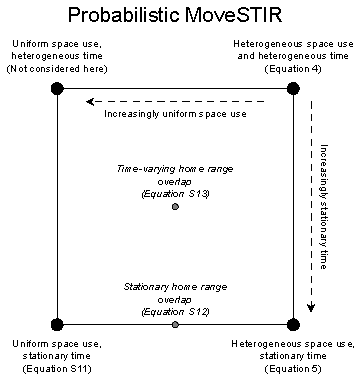
\includegraphics[width=\textwidth]{figures/conceptual_figure_pmovestir.pdf}
    \caption{Conceptual figure for PMoveSTIR}
	\label{fig:square}
\end{figure}

 \begin{figure}
     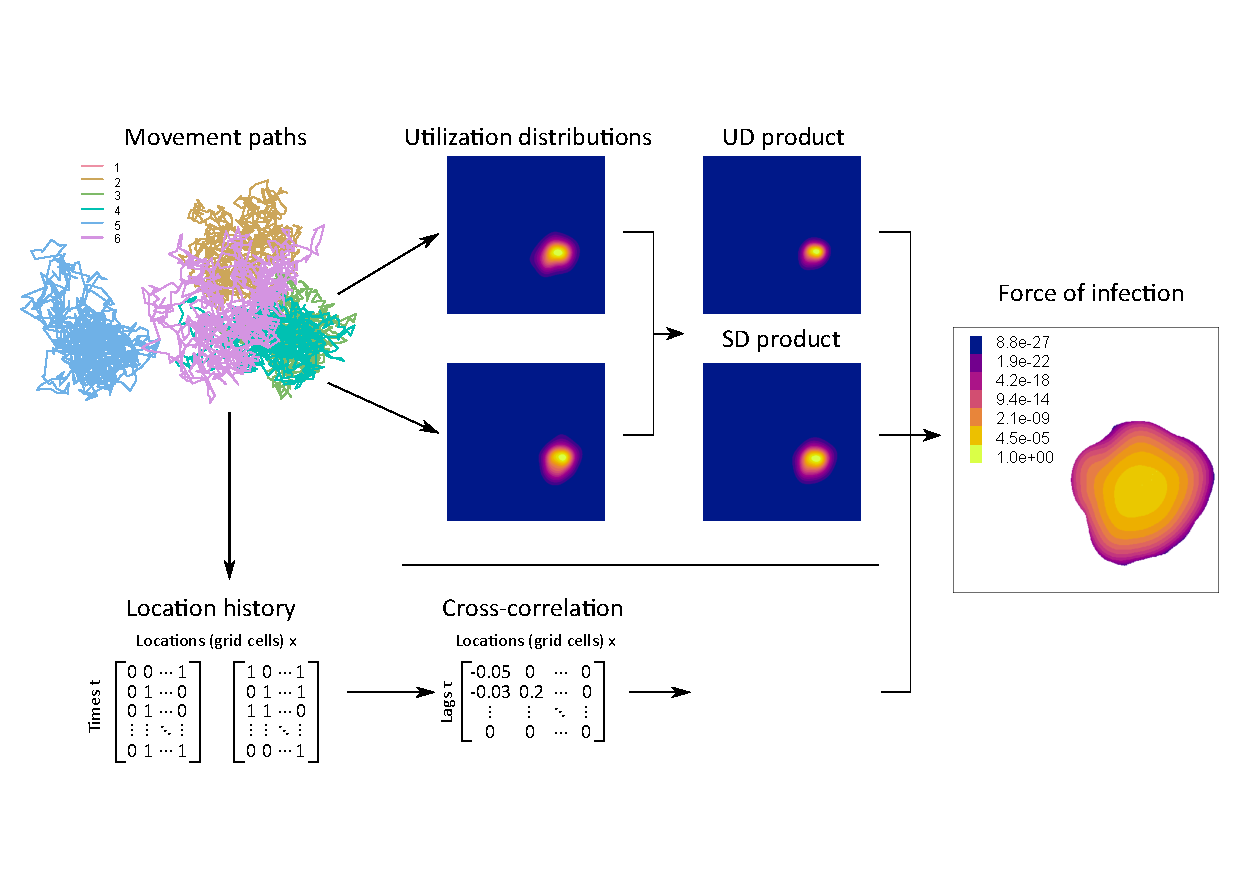
\includegraphics[width=\textwidth]{figures/steps_diagram.pdf}
     \caption{Process to estimate pairwise FOIs using the PMoveSTIR framework assuming stationary utilization distributions}
 	\label{fig:steps}
 \end{figure}

\begin{figure}
    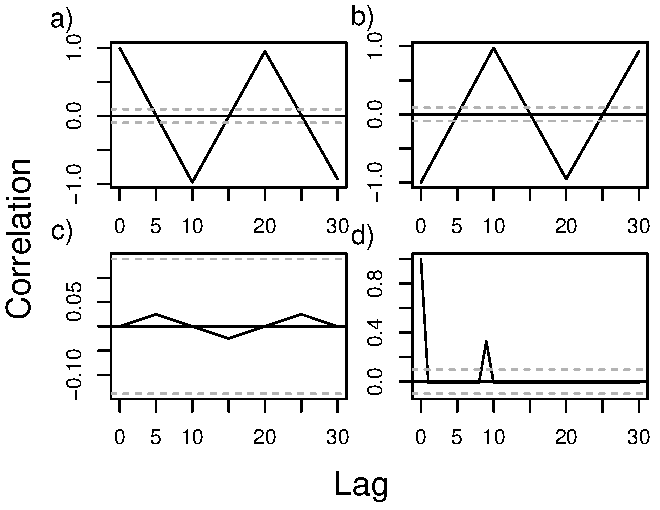
\includegraphics[width=\textwidth]{figures/example_xcorrs.pdf}
    \caption{Variation in cross-correlation values for different combinations of position histories}
	\label{fig:xcorrs}
\end{figure}


\begin{figure}
    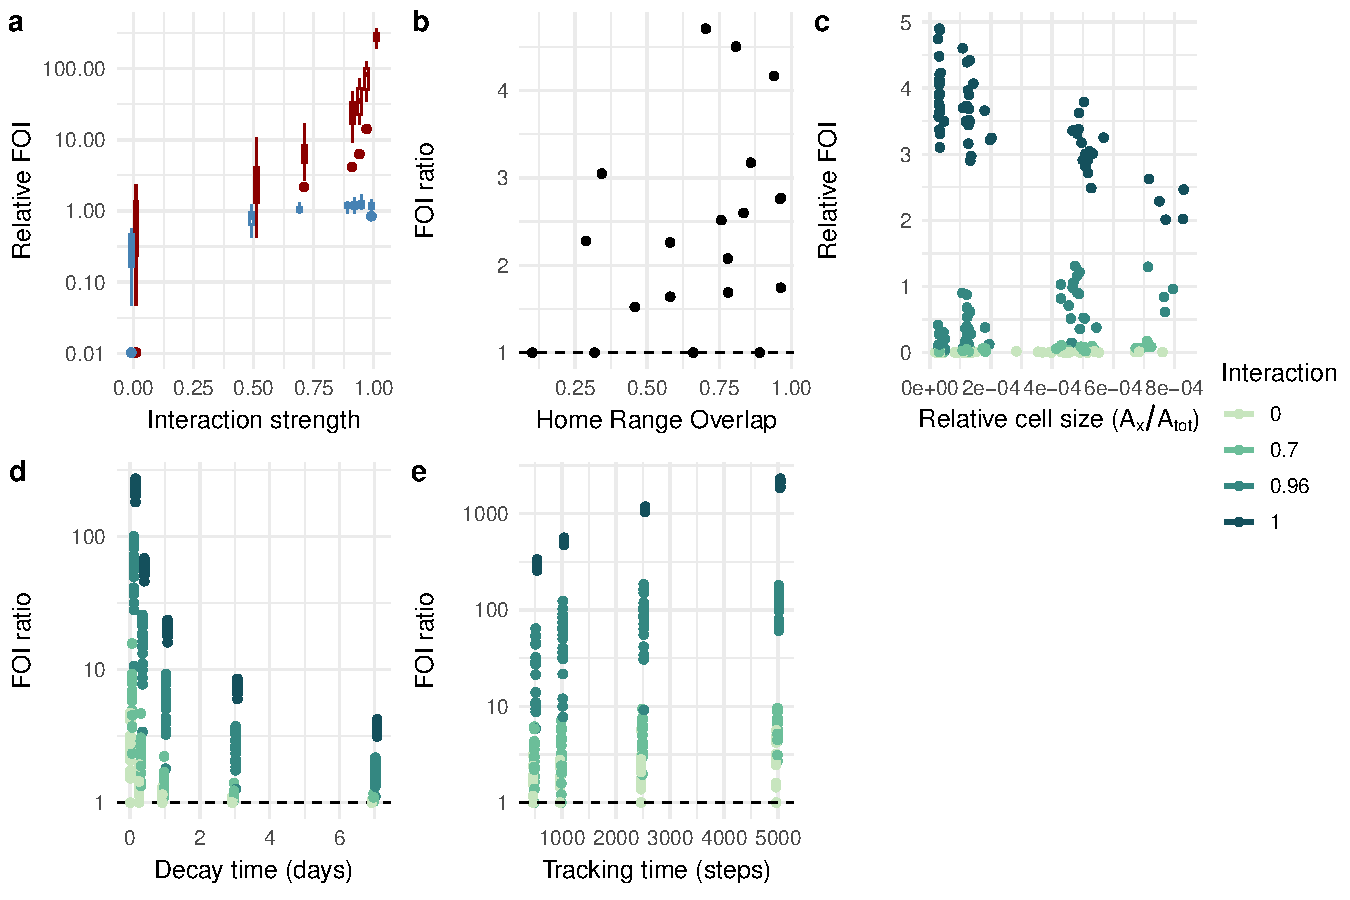
\includegraphics[width=\textwidth]{figures/sim_results.pdf}
    \caption{Analysis of simulated movement data show how the force of infection varies depending on movement processes, namely the strength of attraction between individuals, and how the estimated FOI depends on epidemiological parameters such as the decay rate and threshold distance}
	\label{fig:simresults}
\end{figure}

\begin{figure}
     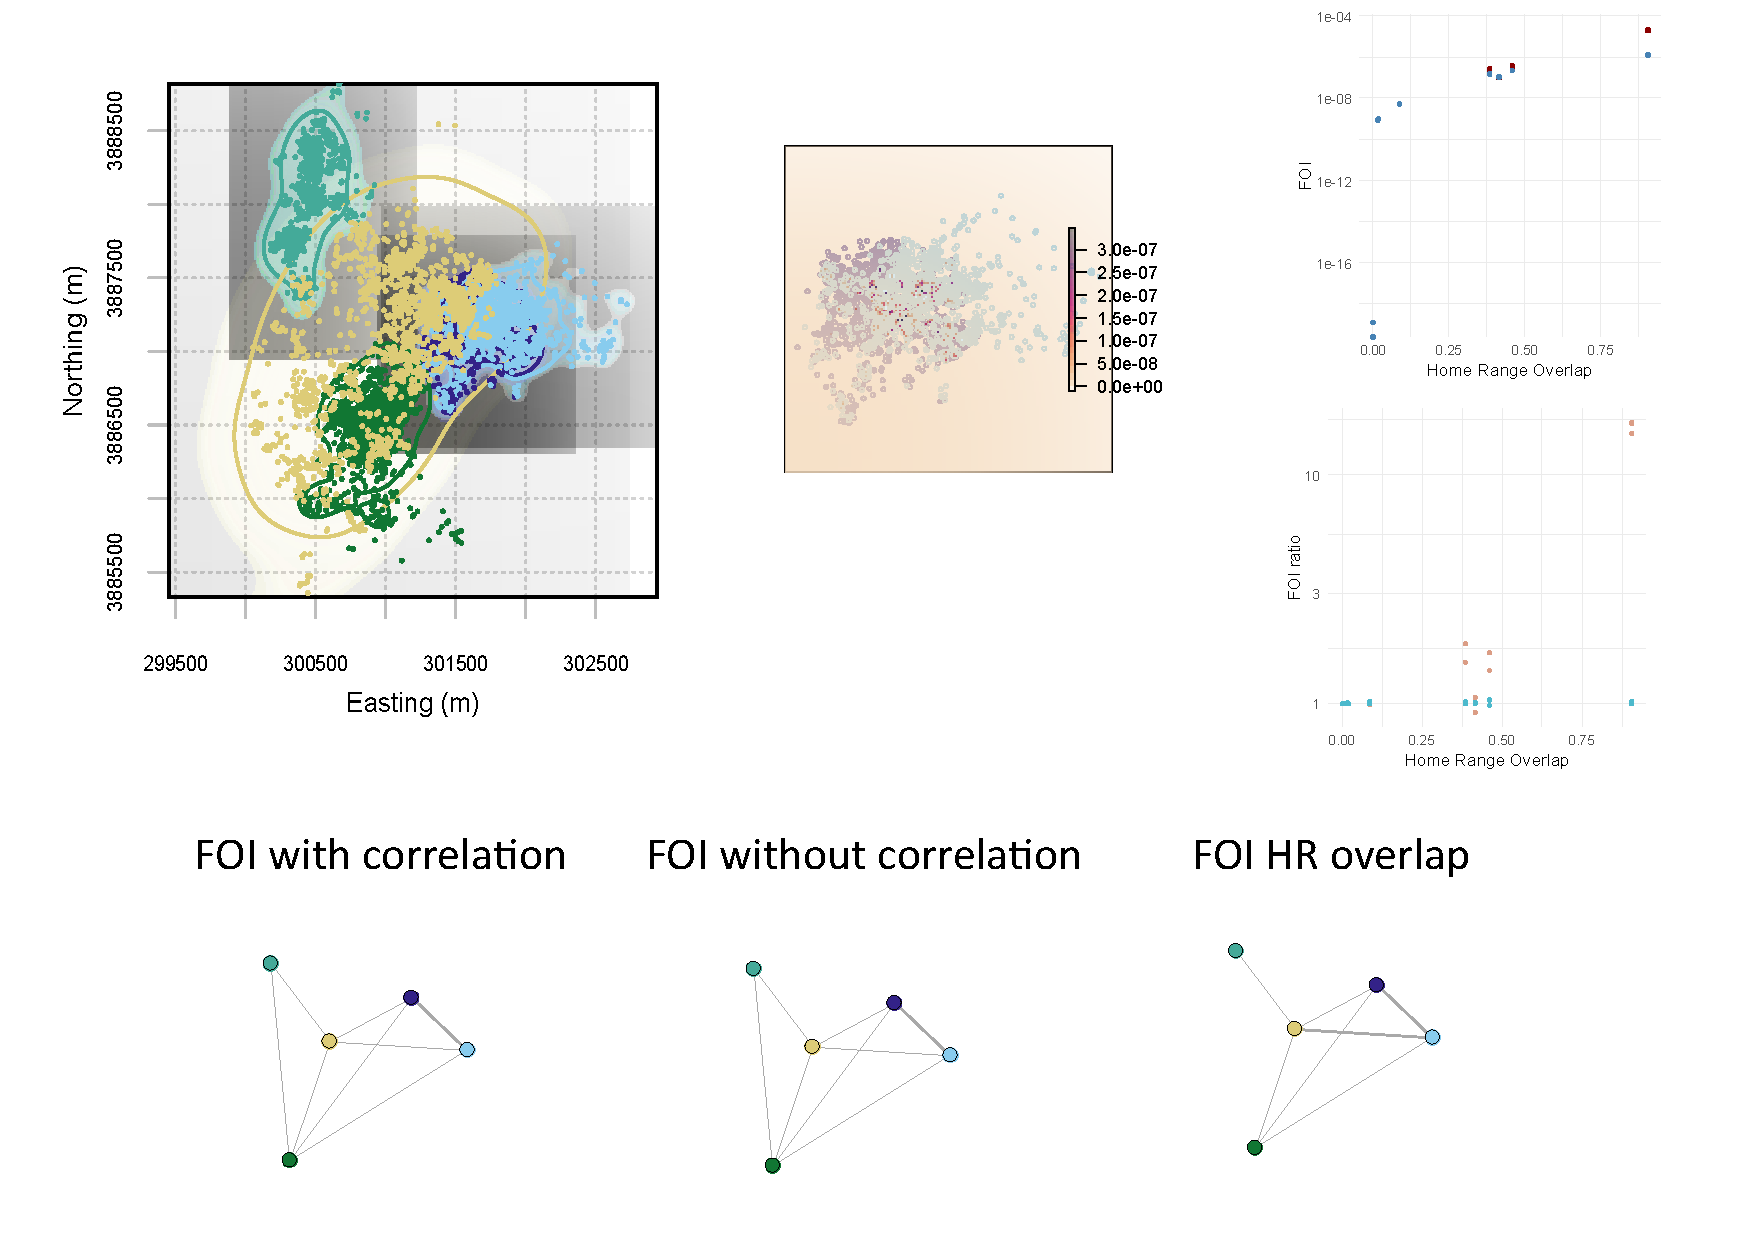
\includegraphics[width=\textwidth]{figures/deer_results.pdf}
    \caption{Empirical FOI estimates from tracking data of white-tailed deer}
	\label{fig:empiricalres}
\end{figure}


\end{document}
